% Chapter 4

\chapter{Linear Control of the Boost Converter} % Main chapter title

\label{Chapter4} % For referencing the chapter elsewhere, use \ref{Chapter1} 

\lhead{Chapter 4. \emph{Control of the Boost Converter}} % This is for the header on each page - perhaps a shortened title

%----------------------------------------------------------------------------------------
In order to better understand the control mechanisms at play in a typical power inverter, we undertook a course of study to learn about the state-of-the-art in DC boost control. The the DC boost circuit is a highly non-linear mechanism, and much of our initial research was into the various mathematical techniques employed to develop linear models of the circuit. Amongst them are the state space averaging technique, circuit linearization via transformation, numerical methods, and small signal analysis.

In the particular case of the DC-DC boost converter circuit shown in Fig. \ref{boost}, the design of a digital or analog controller is complicated by the non-linear nature of the system. From linear control theory, we know that positive gain and phase margins are necessary to ensure the stability of a system in the presence of disturbances. Gain margin can be understood as a safety margin for model uncertainty, while the phase margin provides a safety factor of additional phase lag or lead to ensure system stability. In order to achieve this goal while simultaneously designing for quick response, we set out to study the design of compensators for controlling this class of PWM boost converters. 

Subsequent analysis will show that the transfer function for the DC-DC converter displays unstable characteristics in the presence of a RHP pole. A Bode plot of the system reveals negative gain and phase margins. In order to rectify these unstable characteristics, controllers with proportional-integral control are employed. Compensators are specialized filters designed to provide a specific gain and phase shift at a particular frequency. Because the DC boost circuit introduces a phase lag to the system, we must comprehend this in the design and implementation of our feedback loop. If we performed feedback on a lagging signal without compensation, wild oscillations would likely occur as constructive interference would never result in zero error. 

The hybrid inverter team is interested in this type of control in order to reliably step up DC voltage from a small set of solar panels, and make it a viable source to the hybrid inverter whose output will be targeted at 120VRMS.
Additionally, by changing the voltage reference, we will be able to implement a MPPT algorithm in order to harvest the most energy possible from the panels.

The rest of this paper is structured as follows: in the next section, we will cover the various methods of linearization for the DC boost plant model, as well as the fundamental choice between voltage and current mode operation. Next, we will cover some fundamental topics in control theory, and justify the design of our proportional-integral lag compensator. 

Finally, we will discuss the steps needed to implement the compensator digitally, and cover some of the special considerations of implementation on a micro controller.  

\begin{figure}[htbp]
\begin{center}
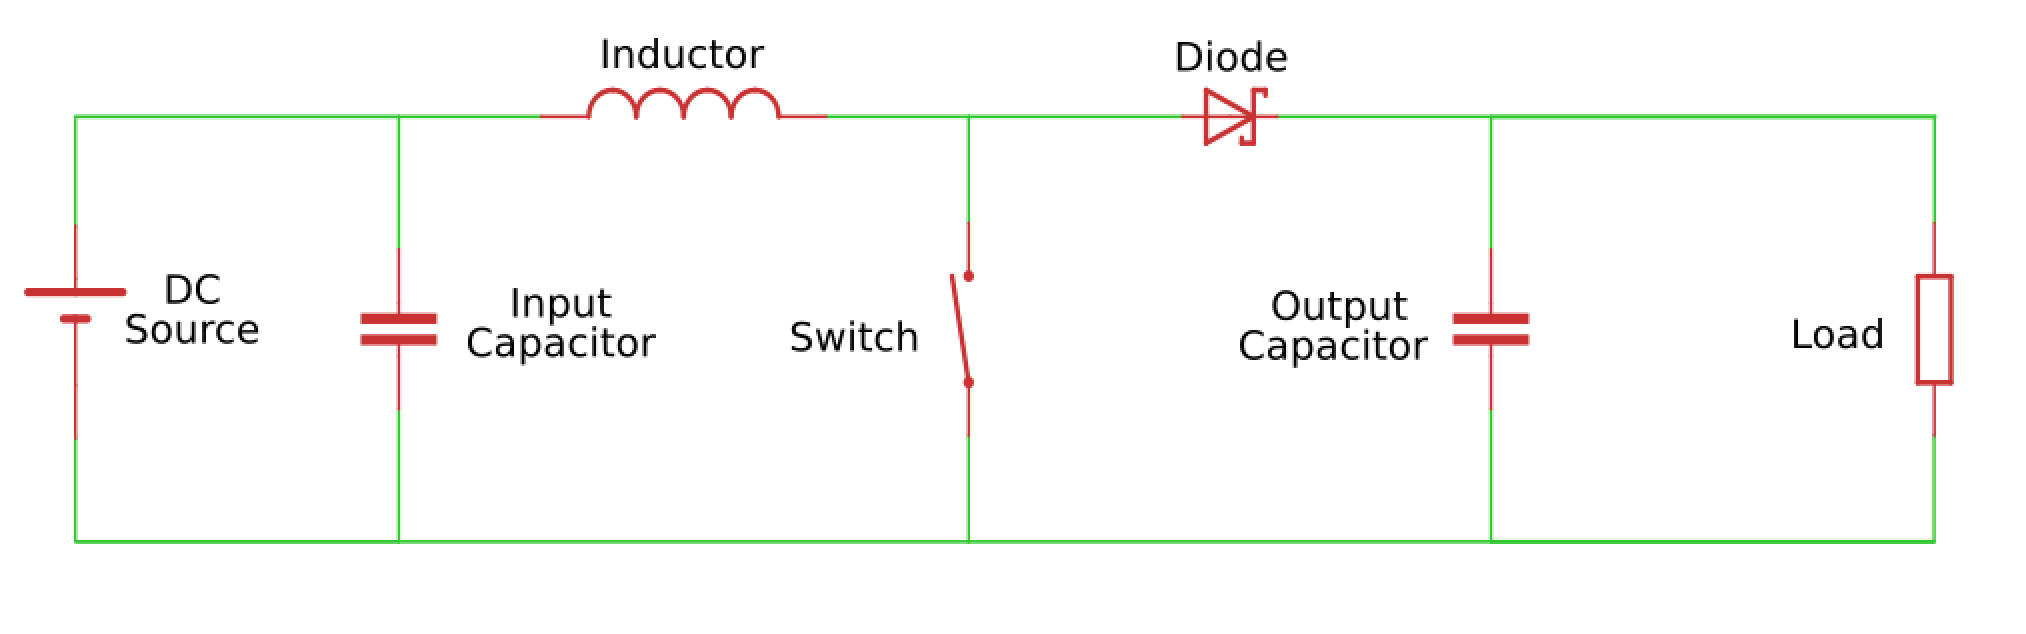
\includegraphics[height = 2.5in, width = \columnwidth]{boostClean}
\caption{The Canonical DC-DC Boost Circuit}
\label{boost}
\end{center}
\end{figure}

%\subsection*{Boost Controller Analysis}

\section{Towards a Linear Model of the DC Boost}

The DC boost circuit in Fig. \ref{boost} has been the subject of countless dissertations dating back to the nineteen seventies. Accordingly, the landscape is a dense one. Fortunately, most researchers agree on a small signal model developed by Dr. Raymond Ridley in the nineties. Ridley's innovation was his synergistic approach, applying both numerical, sampled-data techniques with his current control model. This model employed a linear model of PWM which allowed for the simplified analysis of all SWMPS topologies. This is the model that we've used to develop our controller (see Equation \ref{thirdOrder}). See Equation. For the sake of being thorough, we will cover some alternative methods of analysis and circle-back to a discussion on Dr. Ridley's small signal and modeling approach.

\subsection{Dynamic Averaging}

In \cite{mohan}, a method for modeling the DC boost circuit with an ideal switch, an ideal transformer, and ideal current sources allows for a straightforward analysis using basic circuit analysis. After linearizing the circuit model, perturbation theory is applied to allow for the treatment of the non-linear variables as a sum of DC and AC components. For example, the function $x(t)$ would be represented as $x(t) = X + \tilde{x}$, where $X$ is the DC components, and $\tilde{x}$ is the AC component of the small signal representation. 

The resulting linear equations for $\tilde{v}$ and $\tilde{i}$, the voltage on the output loop and the current through the input loop respectively are given by: 

\begin{equation}
\begin{split}
\tilde{v}_{cp}(t) &= D\tilde{v}_{vp} + V_{vp}\tilde{d} \\
\tilde{i}_{vp}(t) &= D\tilde{i}_{cp} + I_{cp}\tilde{d}
\end{split}
\end{equation}
where the subscripts $vp$ or $cp$ indicate the voltage and current paths respectively. In Mohan's analysis, the boost circuit is split into two loops, the input loop being the current path, the output loop being modeled as the voltage path. 

Finally, the transfer function resulting from this analysis is given by:
\begin{equation}
\label{thirdOrder}
\frac{\tilde{v}}{\tilde{d}} = (1-\frac{sL_e}{R}) \frac{1 + sRC}{L_eC(s^2+s(\frac{1}{RC} + \frac{R}{L_eC}) + \frac{1}{L_eC})}
\end{equation} 

For a duty cycle $D$, effective inductance $L_e$, capacitance C. Note that the effective inductance goes as the inverse square of the prime duty cycle, where the prime duty cycle refers to one minus the duty. 

Mohan's analysis was a useful stepping stone for understanding the basis for circuit linearization and analysis; his concise coverage of the modes of operation seen on DC boost converters, namely, the two DC steady states either off or fully on, and his explanation of discontinuous and continuous conduction regimes were invaluable.

\subsection{State Space Averaging}

Because the DC boost circuit can be viewed as occupying one of two states - off or on - we can view a linearized model of the circuit as being the average of the two states, based on the duty cycle of the PWM. 

For state one where the switch is closed, 
\begin{equation}
\begin{split}
V_s = V_L \\
V_s = L\frac{di}{dt} \\
\frac{di}{dt} = \frac{V_s}{L}
\end{split}
\end{equation}

And state two where the switch is open:

\begin{equation}
\begin{split}
V_s = V_L + V_o\\
V_s = L\frac{di}{dt} + V_O \\
\frac{di}{dt} = \frac{V_s}{L} - \frac{V_o}{L}
\end{split}
\end{equation}

Because the variable duty cycle gives rise to a weighted average, we define the time that the switch is closed as $\delta T_s$ and the time that the switch is open as $(1-\delta)T_s$

So the averaged equations become: 

\begin{equation}
\begin{split}
\dot{i_L} = \frac{1}{T_s}[\delta T_s & \frac{V_s}{L} + (1-\delta)T_s(\frac{V_s}{L} - \frac{V_o}{L})] \\
\dot{i_L} &= \frac{V_s}{L} - \frac{(1-\delta)v_o}{L}
\end{split}
\end{equation}

\begin{equation}
\begin{split}
\dot{v_o} = \frac{-\delta T_s v_o}{RC}& +  (1-\delta)T_s(\frac{i_L}{C} - \frac{v_o}{RC})\\
\dot{v_o} = &\frac{(1-\delta)i_L}{C} - \frac{v_o}{RC}
\end{split}
\end{equation}

With the averaged equations defined, we are free to apply the laplace transform with perturbation terms as above.

\begin{equation}
\begin{split}
\delta(I_L + \hat{i_L})& = \frac{V_s}{L} - \frac{(1-D-\tilde{d})(V_o + \hat{v_o})}{L} \\
\delta(V_o + \hat{v_o}) &= \frac{(1-D-\tilde{d})(I_L \hat{i_L})}{\delta t} - \frac{(V_o +\hat{v_o})}{RC}
\end{split}
\end{equation}
After expansion and elimination:
\begin{equation}
\begin{split}
\hat{\dot{i_L}} = \frac{\hat{\delta}V_o}{L} - &\frac{\hat{v_o}}{L} + \frac{D\hat{v_o}}{L}\\
\hat{\dot{v_o}} = \frac{(1-D)\hat{i_L}}{C}& - \frac{\delta I_L}{C} + \frac{\hat{v_o}}{RC}
\end{split}
\end{equation}
By Laplace transform we arrive at:
\begin{equation}
\begin{split}
\hat{\delta}V_o = sL\hat{i_L} - (1-D)\hat{v_o} \\
\hat{\delta}I_L = \frac{(1-D)\hat{i_L}}{C} - (sC = \frac{1}{R})\hat{v_o}
\end{split}
\end{equation}
Which leads naturally to the state space representation given below:
\begin{equation}
\begin{bmatrix}
V_0  \\ I_L 
\end{bmatrix}
 = 
\begin{bmatrix}
sL & (1-D) \\ 
(1-D) & -(sC + \frac{1}{R}) 
\end{bmatrix}
\begin{bmatrix}
\hat{i_L}  \\ \hat{v_o} 
\end{bmatrix}
\end{equation}

Since we want $\frac{\hat{v_o}}{\delta}$, we take the inverse of the matrix and get

\begin{equation}
\frac{1}{\hat{\delta}}\begin{bmatrix}
V_0  \\ I_L 
\end{bmatrix}= 
\begin{bmatrix}
sL & (1-D) \\ 
(1-D) & -(sC + \frac{1}{R}) 
\end{bmatrix}^{-1}
\begin{bmatrix}
\hat{i_L}  \\ \hat{v_o} 
\end{bmatrix}
\end{equation}

with the inverse matrix given as:
\begin{equation}
A^{-1} = \frac{1}{tf}\begin{bmatrix}
sRC + 1 & R(1-D) \\ 
R(1-D) & -(sC+\frac{1}{R})) 
\end{bmatrix}
\end{equation}

Where
\begin{equation}
tf = s^2RLC + sL + R(1-D)^2
\end{equation}

So we have that 
\begin{equation}
\frac{\hat{V_o}}{\hat{\delta}} = \frac{V_o}{(1-D)} \bigg\{\frac{-sL + R(1-D)^2}{s^2RLC + sL + R(1-D)^2}\bigg\}
\end{equation}
Note the deviation in this result from the previous one obtained by the average dynamic model. We did not utilize this method for designing the feedback loop, but it was a useful and enlightening exercise nonetheless.

\subsection{Numerical Methods in Matlab}

\begin{figure}[htbp]
\begin{center}
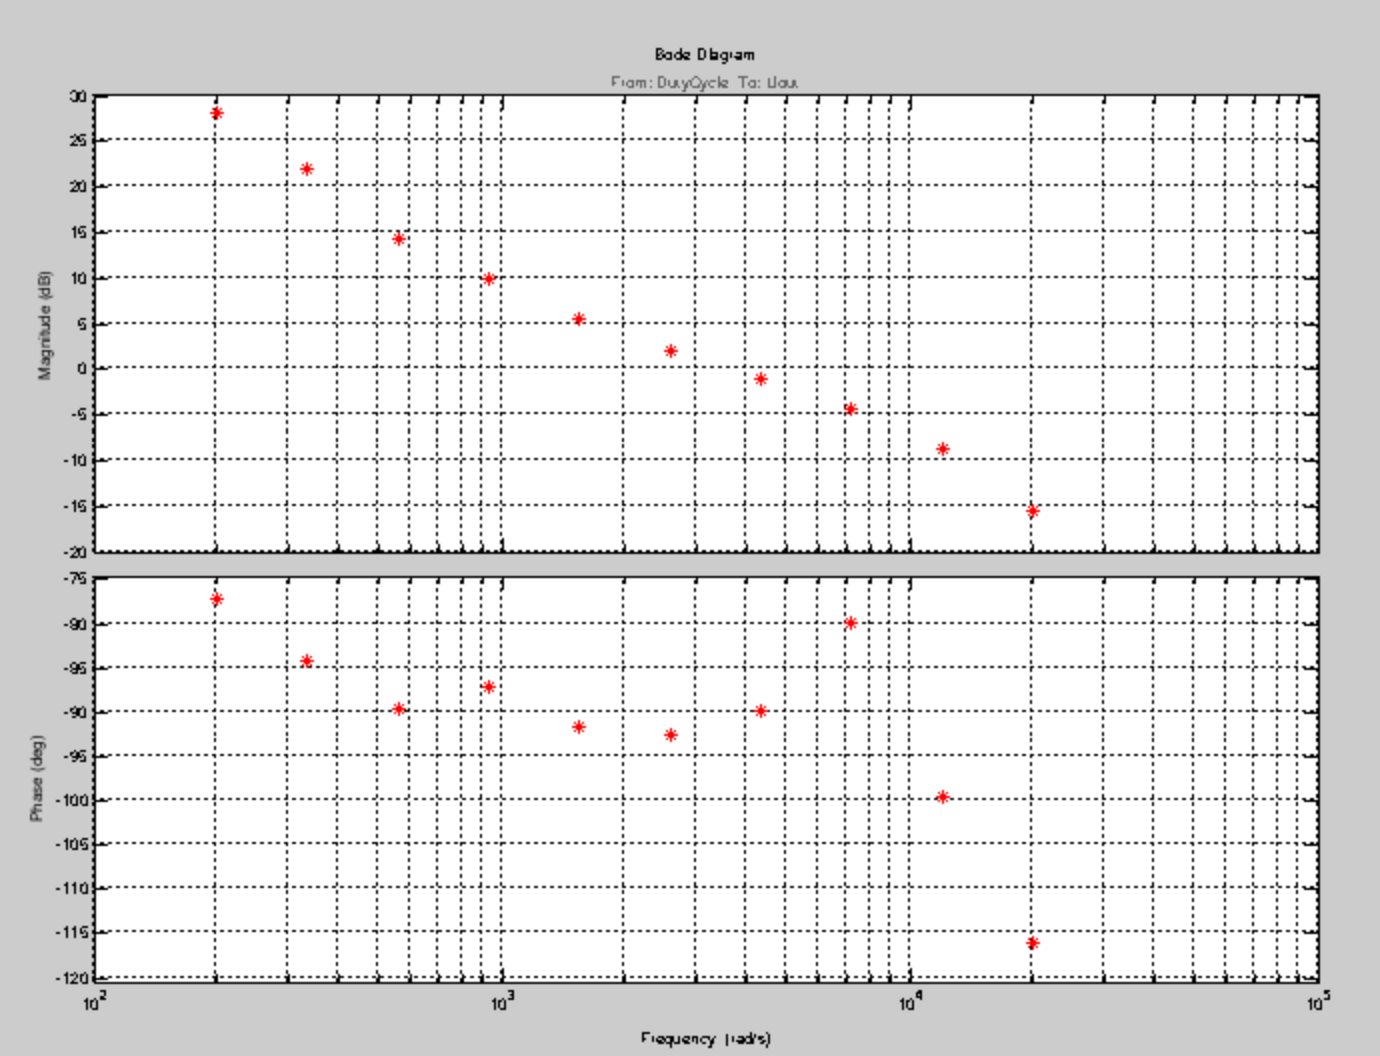
\includegraphics[height = 3in, width = \columnwidth]{prePlant}
\caption{Sampled Data Before Estimation}
\label{prePlant}
\end{center}
\end{figure}
One of the first methods that we used was modeling via simulink. By utilizing an off-the-shelf inverter model, we were able to ascertain the transfer function by following the steps outlined below. 

We began by opening the model below. The $mdl$ variable is reused, so do not omit it.
\begin{verbatim}
	mdl = 'iddemo_boost_converter';
	open_system(mdl);
\end{verbatim}
The frequency response input and output points are created using the $linio$ command and for this example are the outputs of the DutyCycle and Voltage Measurement blocks.
\begin{verbatim}
	ios = [...
	linio([mdl,'/DutyCycle'],1,'input');...
	linio([mdl,'/Voltage Measurement'],
1,'output')];
\end{verbatim}

\begin{figure}[htbp]
\begin{center}
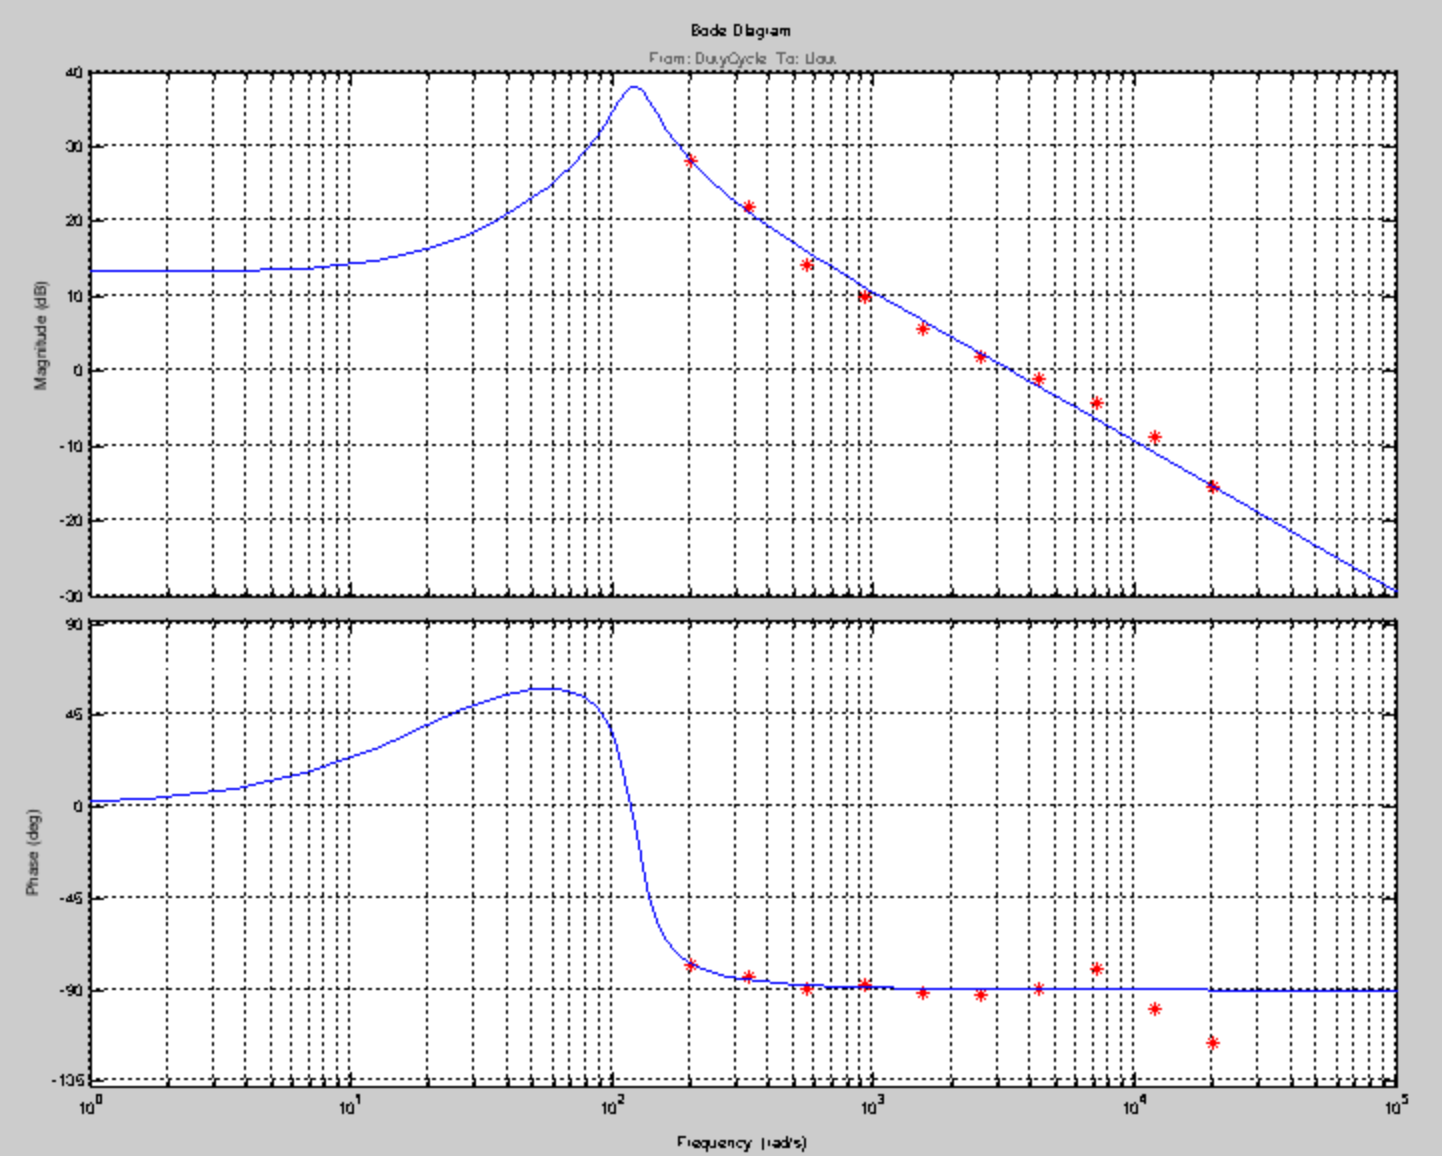
\includegraphics[height= 3in, width = \columnwidth]{plantSimulink}
\caption{Sampled Data with Estimation}
\label{plantSimulink}
\end{center}
\end{figure}

Use the frest.Sinestream command to define the sinusoids to inject at the input point. We are interested in the frequency range 200 to 20k rad/s, and want to perturb the duty cycle by 0.03. After the following commands are entered, the Bode plot of the estimated transfer function is shown as above in Fig. \ref{plantSimulink}. This series of commands is given as follows:

\begin{verbatim}
	f = logspace(log10(200),
         log10(20000),10);
	in = frest.Sinestream('Frequency',
         f,'Amplitude',0.03);
\end{verbatim}

\begin{verbatim}
	getSimulationTime(in)/0.02
\end{verbatim}

\begin{verbatim}
	[sysData,simlog] = 
         frestimate(mdl,ios,in);
	bopt               = bodeoptions;
	bopt.Grid          = 'on';
	bopt.PhaseMatching = 'on';
	figure, bode(sysData,'*r',bopt)
\end{verbatim}

\subsection{Small Signal Analysis}
After a bit of derivation, we arrive at our final point of analysis, the small signal model proposed by Dr. Ray Ridley in his PhD dissertation circa 1990. Using a combination of the technique describes above, Dr. Ridley was able to come up with a linear model of the PWM block that could be used alongside numerical methods. The resulting Transfer function has proven to be the most accurate and reliable for designers of SWMPS. Before we jump into his methods, We'd like to touch on the two fundamental methods for controlling the DC boost circuit.
 
\begin{figure}[htbp]
\begin{center}
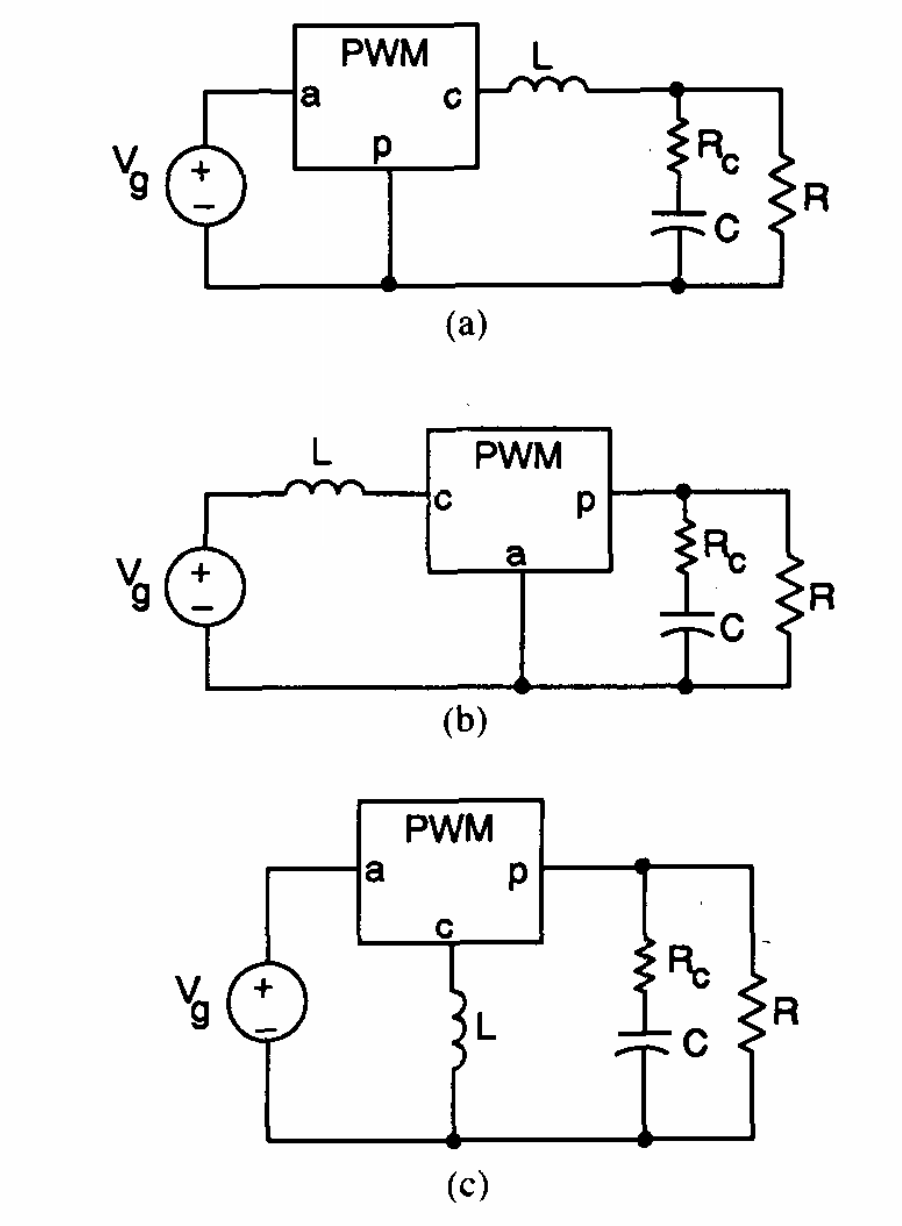
\includegraphics[height= 2.5in, width=4in]{pwmModel}
\caption{Linearized Model of the PWM per Ridley\cite{ridley}}
\label{pwmModel}
\end{center}
\end{figure}

The first method is known as voltage mode control, and as its name implies, relies on voltage feedback from the boost circuits output to regulate itself. This technique is problematic for a few reasons. Changes in the loading condition of the circuit must be sensed as an output change first, then get corrected by the feedback loop. This delay results in slow response. Next, The output filter contributes two poles to the control loop requiring either a dominant pole for low frequency roll-off at the error amplifier, or an added zero in compensation.
Lastly, compensation is complicated by the fact that the loop gain varies with the input voltage.

The preferred controller for the DC/DC boost is the so-called current mode controller; it operates by sensing current through the inductor, or through the FET switch. This method has the advantage over voltage mode control, in that as its inductor current rises with a slope determined by $(V_{in}-V_o)$, the waveform will respond immediately to line voltage changes eliminating the delayed response and gain variation with changes to the input voltage. Additionally, since the error amplifier if now used to command an output current rather than an output voltage, the effect of loading is minimized and only a single pole is contributed to the feedback loop. This allows for simpler compensation and higher bandwidth over a comparable voltage mode controller. 

Dr. Ridley's model is designed with current mode control in mind. His analysis shows that the transfer function of a boost converter is found to be:

\begin{equation}
f_p(s)=\frac{k[1 + \frac{s}{\omega_z}][1 - \frac{s}{\omega_{z,RHP}}]}{[1 + \frac{s}{\omega_p}]}
\end{equation}

Where $\omega_p = \frac{2}{RC}$, ~$\omega_z = \frac{1}{R_cC}$, ~$R_c$ is the ESR of the cap, and $\omega_{z,RHP} = \frac{R(1-D)^2}{L}$.

The difference between the average inductor current and the dc value of the sampled inductor current can cause instability for certain operating conditions. This instability is known as sub-harmonic oscillation, which occurs when the inductor ripple current does not return to its initial value by the start of next switching cycle. These oscillations are characteristic of boost circuits using current mode control. Sub-harmonic oscillation is normally characterized by observing alternating wide and narrow pulses at the switch node. This term contributes to the total transfer function and is given by:

\begin{equation}
f_h(s)=\frac{1}{\frac{s^2}{w_n^2} + \frac{s}{w_nQ_p} + 1}
\end{equation}

We summarize their constituent expressions here:

\begin{gather*}
m_c = 1 + \frac{s_e}{s_n} \\
s_e = \frac{Vpp}{Ts} \\
s_n = \frac{Von}{L} \\
\omega_n = \frac{\pi}{Ts}\\
Q_p = \frac{1}{\pi(m_cD^{'}-1/2)}
\end{gather*}

Where $V_{on}$ is the inductor voltage with the switch on, and $R_i$ is the gain from the inductor current, implying that $R_i$ is the sense resistor.

Therefore, the total transfer function given by Ridley in \cite{ridley} is found to be:

\begin{equation}
\label{thirdOrder}
f_p(s)f_h(s)=\frac{k[1 + \frac{s}{w_z}][1 - \frac{s}{w_{z,RHP}}]}{[1 + \frac{s}{w_p}][\frac{s^2}{w_n^2} + \frac{s}{w_nQ_p} + 1]}
\end{equation}

From here, we are ready to analyze the resultant Bode plot to determine what type of compensation will be necessary for this plant model. This plot is shown below in Fig.\ref{plantModelRidley}.
The poles and zeros are placed in such a way that the system has enough phase margin, and to minimize the effect of maximum phase lag due to a Right-Half plane zero.

\begin{figure}[htbp]
\begin{center}
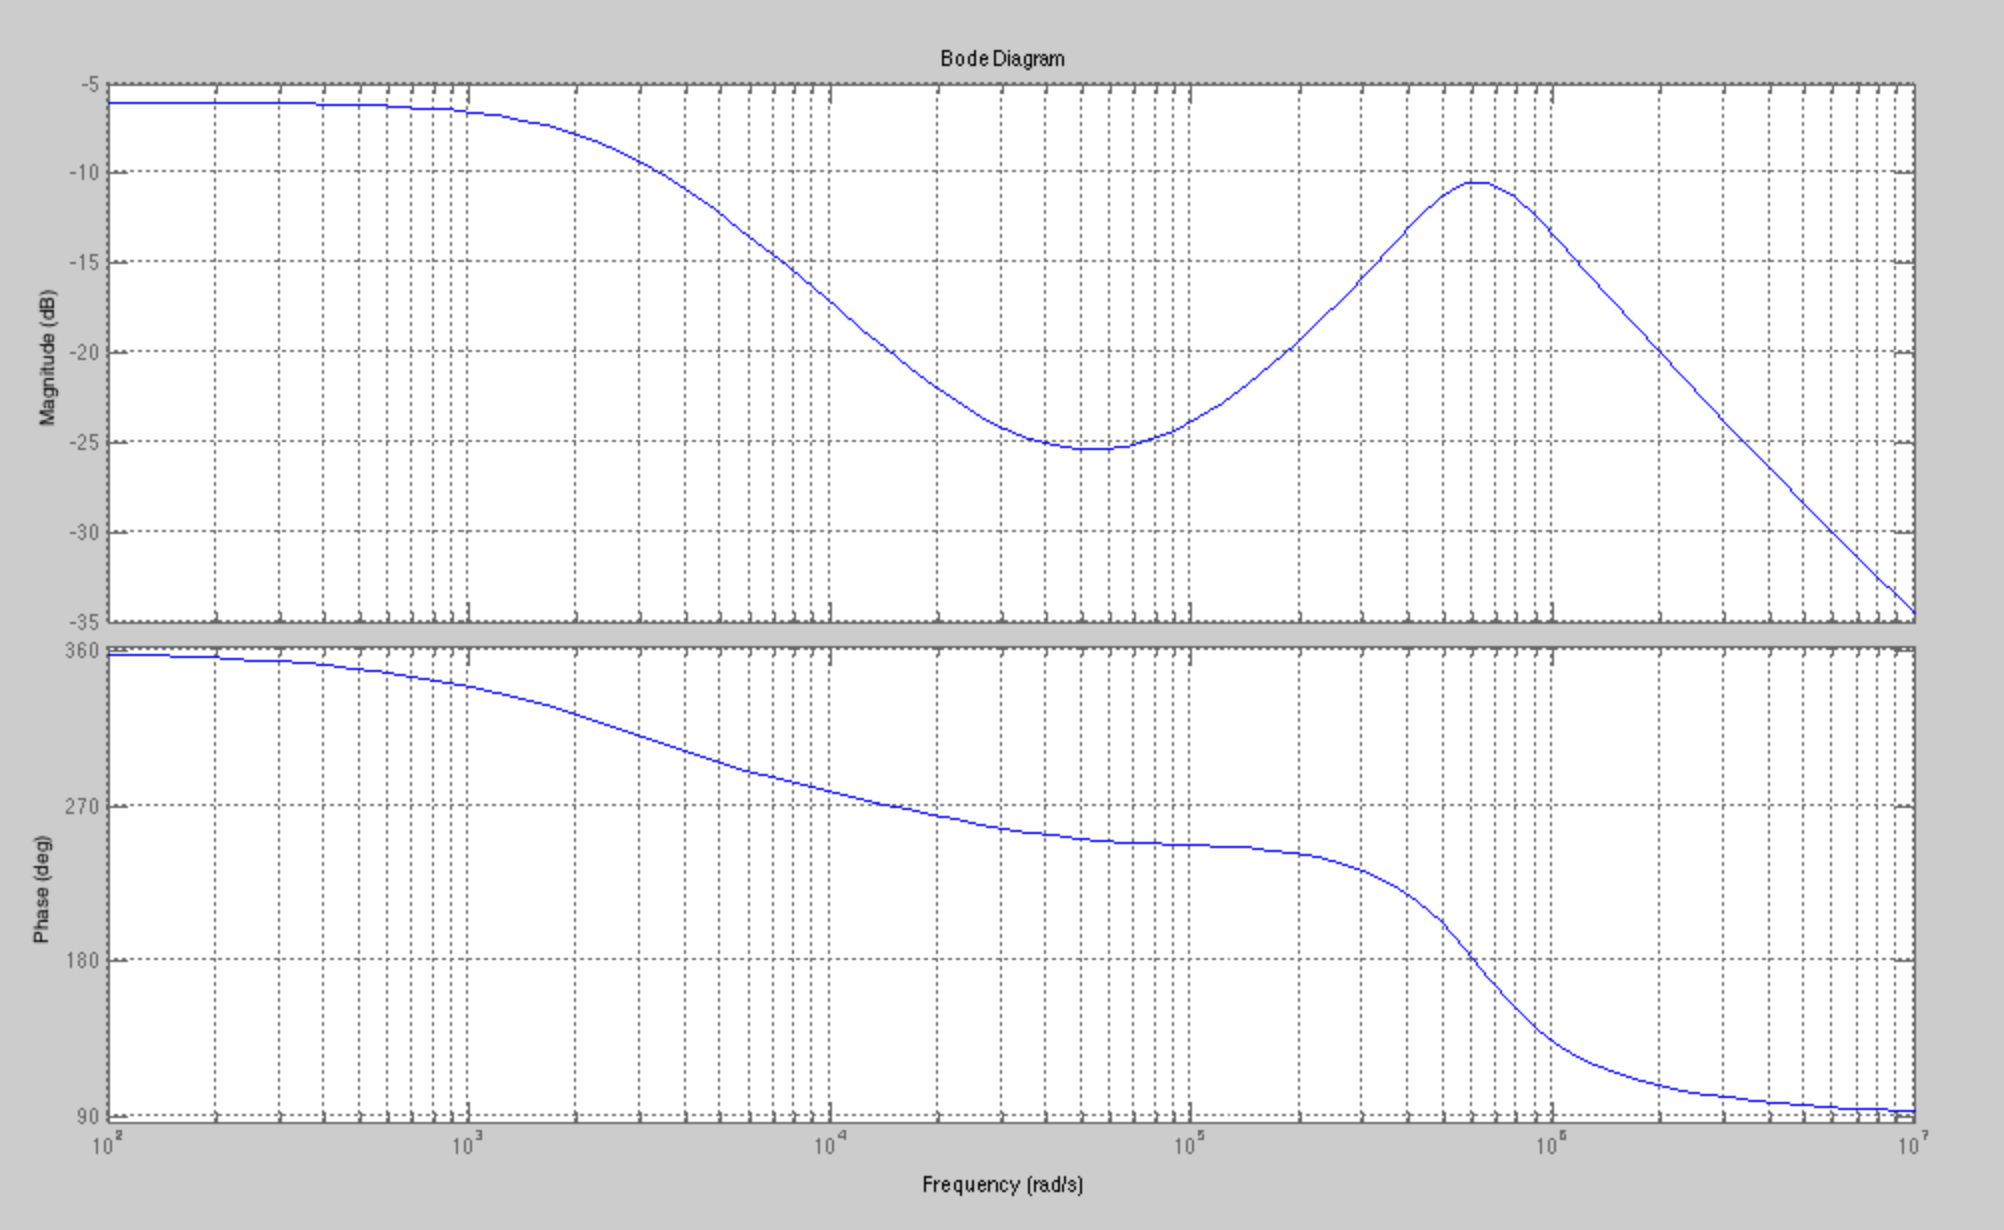
\includegraphics[height= 3in, width = \columnwidth]{plantModelRidley}
\caption{The total transfer function $f_p(s)f_h(s)$ for the DC boost circuit}
\label{plantModelRidley}
\end{center}
\end{figure}

From \cite{mohan}, we have that a compensator for this system in current mode control is given by
\begin{equation}
G_c(s) = \frac{k_c(1 + \frac{s}{\omega_z})}{s(1+\frac{s}{\omega_p})}
\end{equation}
Choosing our desired phase margin to be $\phi_{boost} = 60^{\circ}$, we have that our key parameters are:
\begin{gather*}
k_{boost} = tan(45^{\circ}+\frac{\phi_{boost}}{2})\\
f_z = \frac{f_c}{k_{boost}}\\
f_p = f_ck_{boost}\\
k_{c} = \frac{\omega_z}{|G_{ps}(s)|_{f_c}}\\
\end{gather*}

By selecting a resonable crossover frequency $f_c$, we can calculate the require parameters of this expression. The resulting compensator is shown in Fig. \ref{lagRidley}.
\begin{figure}[htbp]
\begin{center}
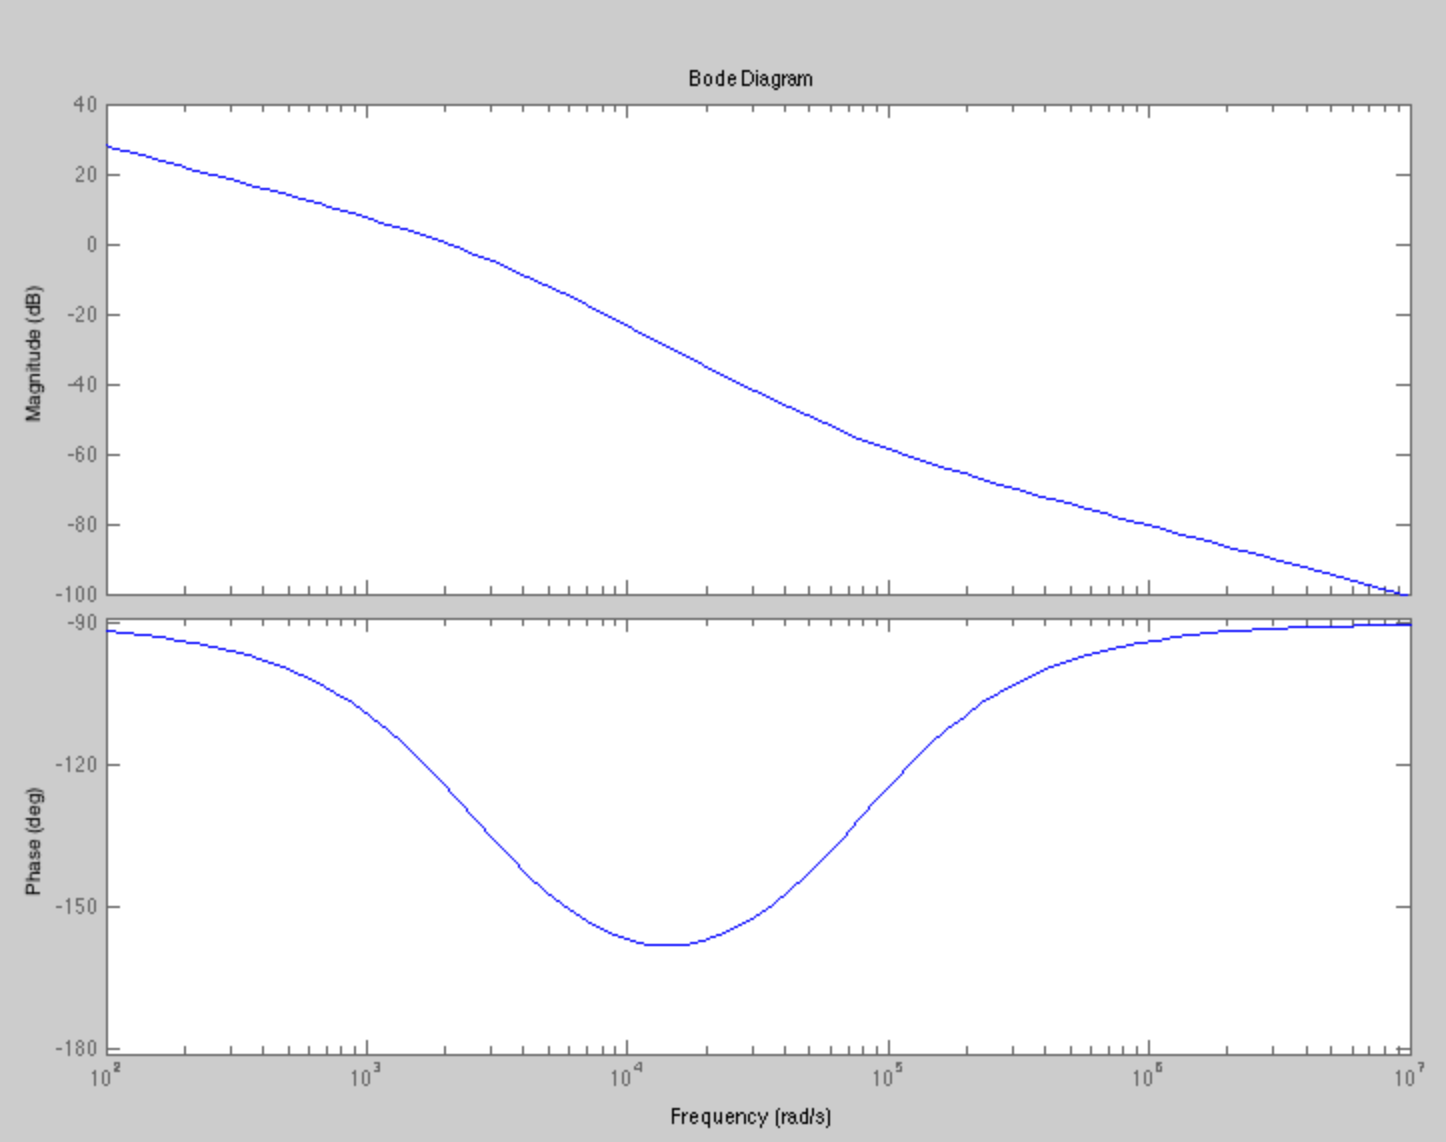
\includegraphics[height= 3in, width = \columnwidth]{lagRidley}
\caption{The lag compensator for the DC boost circuit}
\label{lagRidley}
\end{center}
\end{figure}
Finally, calculating the closed-loop with compensator, we get the stabilized system shown in the third panel of Fig. \ref{composite}. 

\begin{figure}[htbp]
\begin{center}
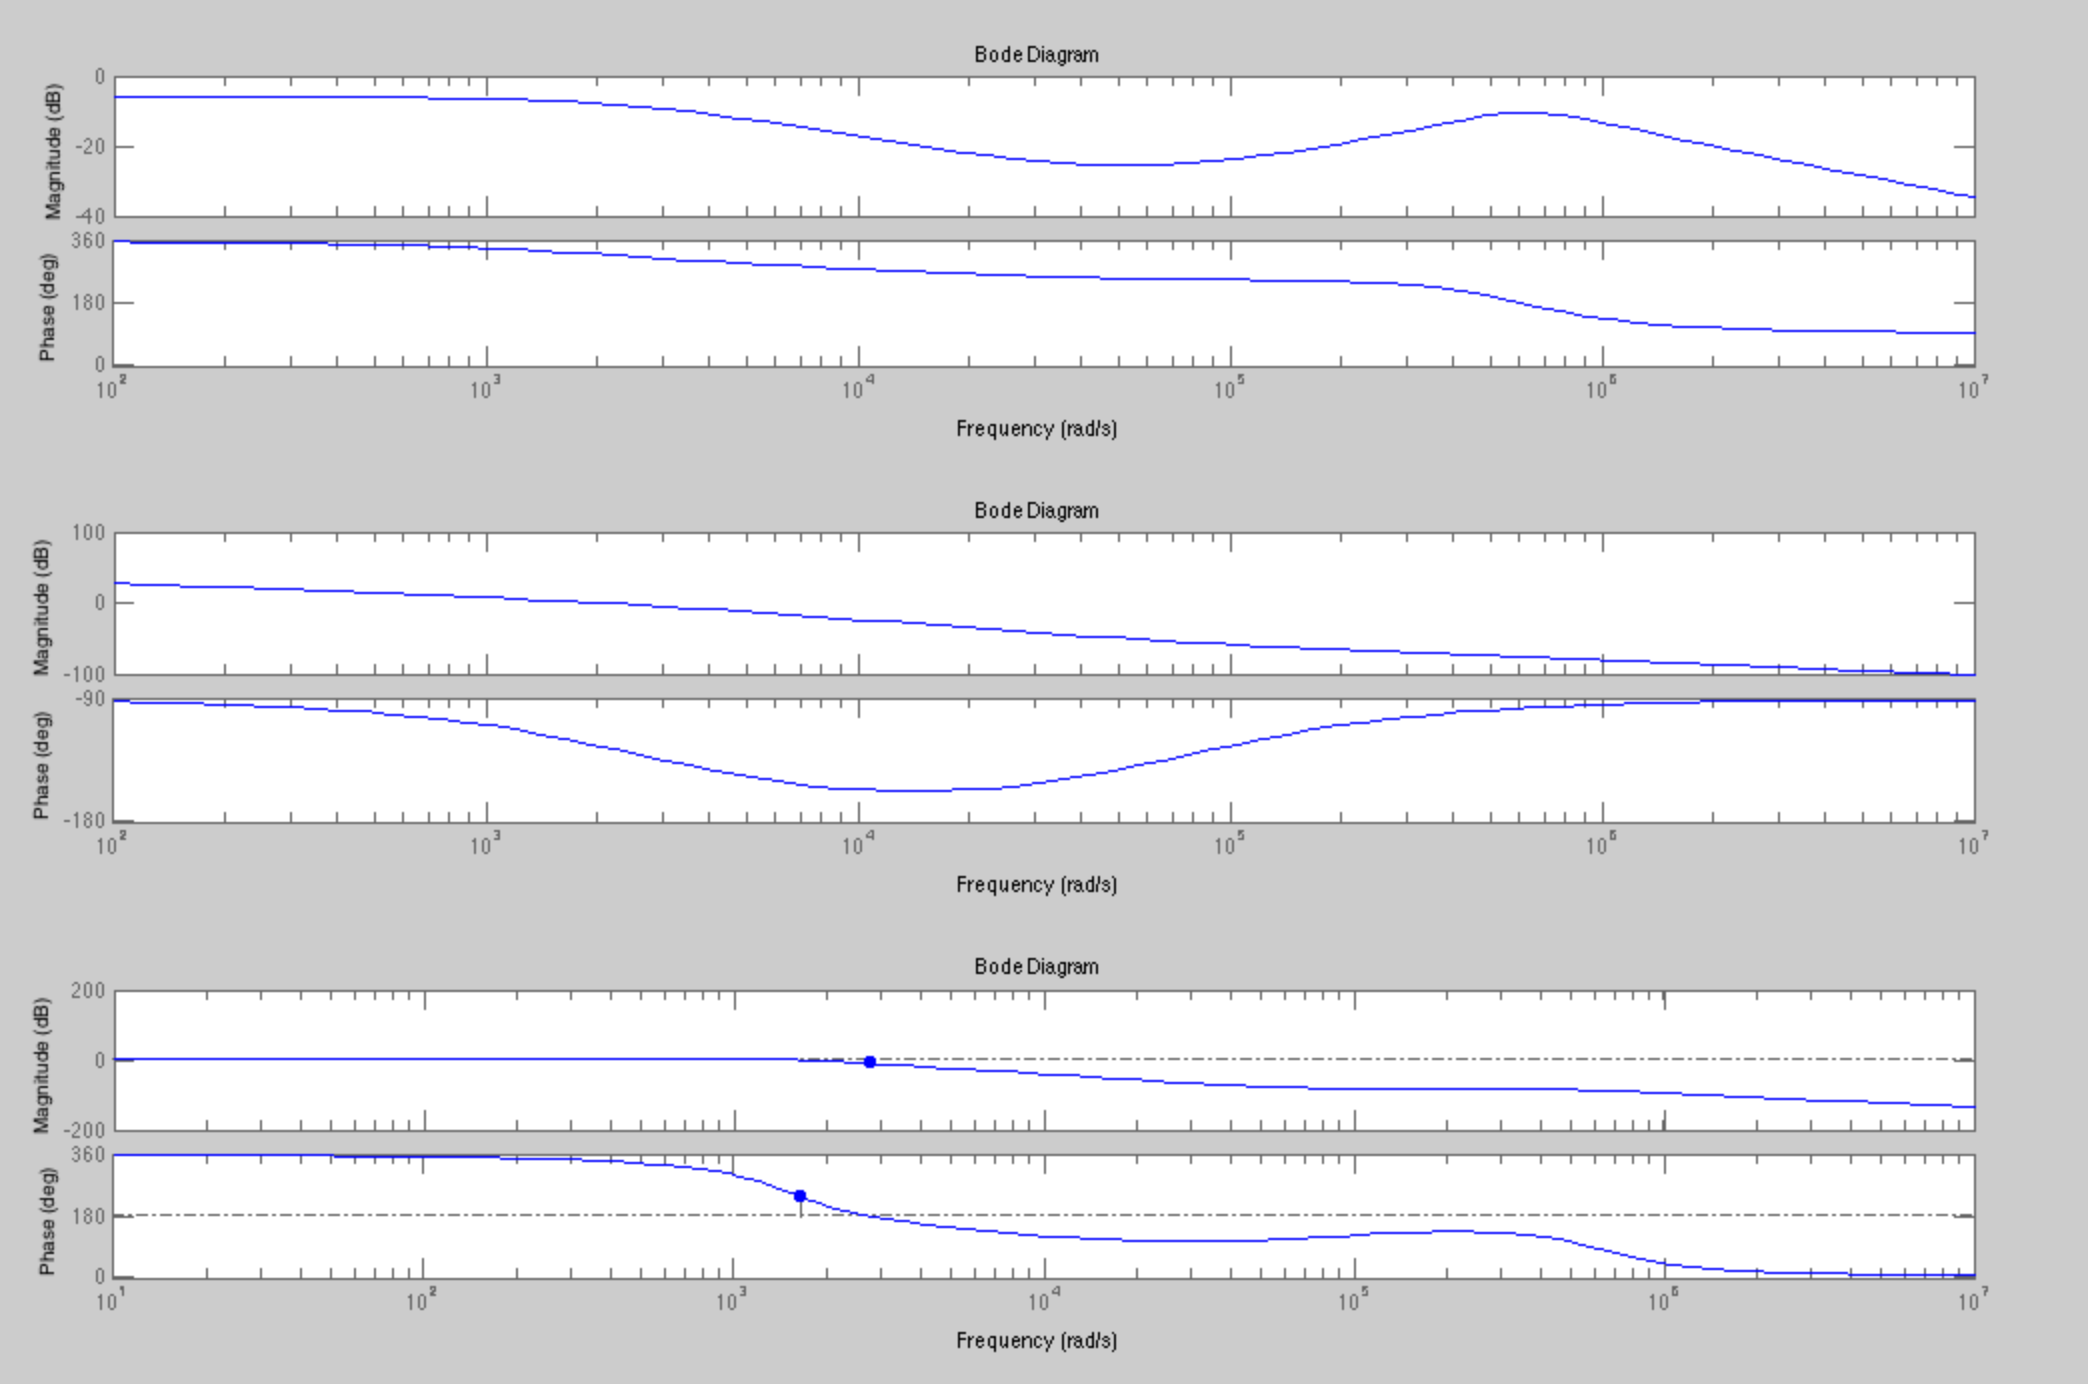
\includegraphics[height= 4in, width = \columnwidth]{composite}
\caption{The Plant, Compensator, and Closed Feedback Loop Bode Plots for the DC boost circuit}
\label{composite}
\end{center}
\end{figure}

For a closer inspection, see Fig. \ref{gpMargin} which clearly shows the gain and phase margins make for a stable system. 

\begin{figure}[htbp]
\begin{center}
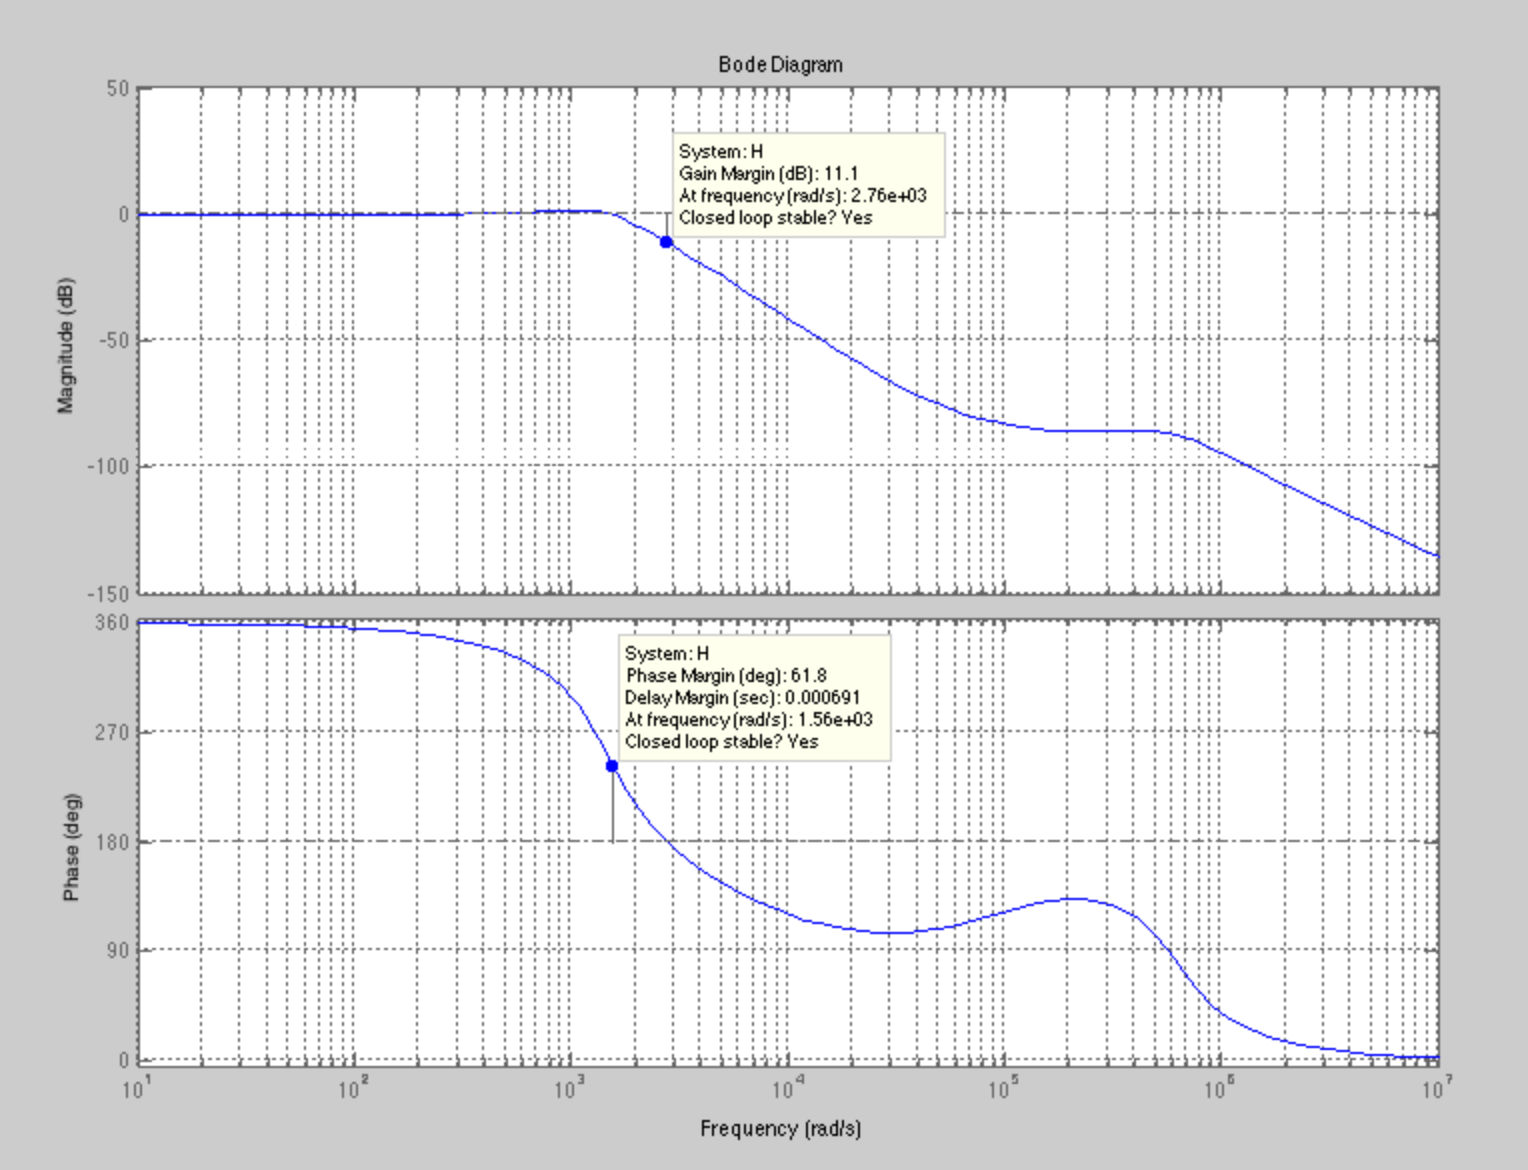
\includegraphics[height= 4in, width = \columnwidth]{gpMargin}
\caption{Bode plot of the closed loop transfer function with gain and phase margin labels}
\label{gpMargin}
\end{center}
\end{figure}

\section{2P2Z}
As we can see, the lag compensator was simply a special case of PI control. A 2P2Z can implement the continuous time version by way of a bilinear or Tustin transformation. The rule for the bilinear transform is that $s\leftarrow\frac{2z-1}{Tz+1}$, Performing this transformation on our controller equation results in an expression of the same form, implementable in assembly on a C2000 Piccolo micro controller by TI. The Biricha tool recommended by TI takes the position of poles and zeroes and convertes them to the necessary coefficients for the micro.

\section{Concluding Remarks on the Boost Controller}
After a fairly exhaustive review of the literature regarding the accuracy of the linearized DC boost model, and the control theory behind their employment in SWMPS, We were able to get favorable results in simulation, namely a stable system. While there are multiple methods for linearizing the boost circuit, the most widely accepted models today utilize of Dr. Ridley's due to its highly accurate predictions. This model was used in the design of a lag compensator. The Final phase involved the conversion of our linear model to a discrete model suitable for implementation on a micro controller.